\documentclass{article}

\usepackage{amsmath}
\usepackage{tikz}
\usetikzlibrary{shapes.geometric, arrows, external}
\tikzexternalize % activate!

\tikzstyle{block} = [rectangle, minimum width=3cm, minimum height=1cm, text centered, draw=black, fill=orange!30, text width=3.5cm]
\tikzstyle{arrow} = [thick,->,>=stealth]
\tikzset{external/force remake}
\begin{document}


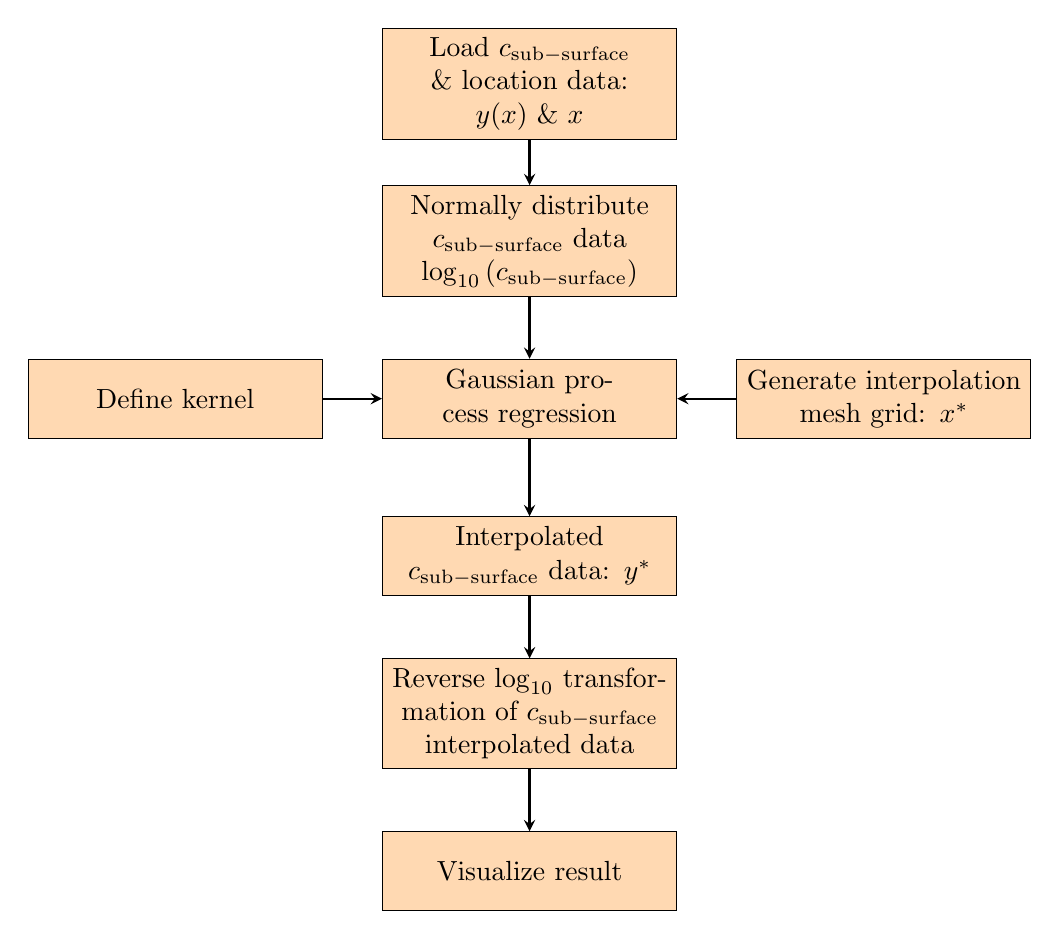
\begin{tikzpicture}[node distance=2cm]

\node (load_data) [block] {Load $c_\mathrm{sub-surface}$ \& location data:\\$y(x)$ \& $x$};
\node (log10) [block, below of=load_data] {Normally distribute $c_\mathrm{sub-surface}$ data $\log_{10}{(c_\mathrm{sub-surface})}$};
\node (regression) [block, below of=log10] {Gaussian process regression};
\node (mesh_grid) [block, right of=regression, xshift=2.5cm] {Generate interpolation mesh grid: $x^*$};
\node (kernel) [block, left of=regression, xshift=-2.5cm] {Define kernel};
\node (output) [block, below of=regression] {Interpolated $c_\mathrm{sub-surface}$ data: $y^*$};
\node (reverse_log10) [block, below of=output] {Reverse $\log_{10}$ transformation of $c_\mathrm{sub-surface}$ interpolated data};
\node (visualize) [block, below of=reverse_log10] {Visualize result};

\draw [arrow] (load_data) -- (log10);
\draw [arrow] (log10) -- (regression);
\draw [arrow] (mesh_grid) -- (regression);
\draw [arrow] (kernel) -- (regression);
\draw [arrow] (regression) -- (output);
\draw [arrow] (output) -- (reverse_log10);
\draw [arrow] (reverse_log10) -- (visualize);

\end{tikzpicture}

\end{document}
